%!TEX root = ../thesis.tex

% FIGURE: detector
% https://cms-docdb.cern.ch/cgi-bin/PublicDocDB/ShowDocument?docid=12201
\begin{figure*}[b!]
  %\vspace{3mm}
  \centerline{
    \includegraphics[width=0.92\textwidth,clip,trim={0mm 12.3mm 0mm 0mm}]{fig/detector/CMS_detector_white.pdf}
  }
  \caption{
The CMS detector.
Taken from~\cite{CMS}.
  } \label{fig:CMS}
  %\vspace{-3mm}
\end{figure*}

% FIGURE: coordinate system & eta
\begin{figure*}[b!]
  %\vspace{2mm}
  \centering
  \centerline{
    \raisebox{-0.5\height}{\includegraphics[width=0.7\textwidth,page=4]{fig/detector/CMS_coordinate_system.pdf}}
    \quad
    \raisebox{-0.4\height}{\includegraphics[width=0.32\textwidth]{fig/detector/pseudorapidity_eta_theta.pdf}} 
  }
  %\vspace{-1mm}
  \caption{
\Left: The conventional coordinate system of CMS with momentum vector $\myvec{p}$.
Taken from~\cite{CMS_coordinate_system}.
\Right: Pseudorapidity.
Taken from~\cite{pseudorapidity}.
  } \label{fig:CMS_coordinate_system}
  %\vspace{-3mm}
\end{figure*}